%==============================================================================
%  Paper 2 -- BAN DUNG LAI (2026-09-21)
%
%  Khac ban da nop IJNM bon diem, tat ca ve DO DAC chu khong ve mo hinh:
%    1. Chi so. ECE tren tap con MOT lop suy bien thanh 1 - trung binh(p), nen
%       ECE_rare cua ban cu khong do calibration. Chi so chinh doi sang ECE
%       tren toan tap test, noi co ca hai lop.
%    2. Tap test. KDDTest+ day du thay vi mot mau 100 dong (10 hiem).
%    3. So run. 10 thay vi 5 -- voi 5 cap, Wilcoxon khong bao gio dat p<0.05.
%    4. Khong dung model cache: moi baseline huan luyen lai tren CUNG mot tap.
%  Cong them UNSW-NB15, chay ca 4 lan 6 qubit de go confound.
%
%  Khoi tac gia giu nguyen ban da nop.
%  Compile: pdfLaTeX. Moi con so phai goi qua macro trong tables/.
%==============================================================================
\documentclass[journal]{IEEEtran}

\usepackage{cite}
\usepackage{amsmath,amssymb,amsfonts}
\usepackage[T1]{fontenc}
\usepackage{newtxtext,newtxmath}
\usepackage{graphicx}
\usepackage{booktabs}
\usepackage{url}
\usepackage[hidelinks]{hyperref}

\newcommand{\QSVM}{QSVM}
\newcommand{\ZZ}{\textsf{ZZ}}
\newcommand{\ECE}{\mathrm{ECE}}
\newcommand{\Brier}{\mathrm{Brier}}

% Sinh boi runners/make_p2_rebuild_tables.py -- dung sua tay.
% Prose KHONG duoc viet so truc tiep; dung macro o day.
\newcommand{\pnRuns}{10}
\newcommand{\pnTest}{22\,544}
\newcommand{\pnRare}{2\,952}
\newcommand{\pnRareOld}{10}
\newcommand{\pnTestOld}{100}
\newcommand{\pnTrain}{1\,000}
\newcommand{\pQsvmEceRare}{0.5414}
\newcommand{\pQsvmEceRareSd}{0.0443}
\newcommand{\pQsvmBrierRare}{0.4323}
\newcommand{\pQsvmBrierRareSd}{0.0488}
\newcommand{\pQsvmAucPr}{0.9332}
\newcommand{\pQsvmAucPrSd}{0.0083}
\newcommand{\pQsvmFone}{0.7982}
\newcommand{\pQsvmFoneSd}{0.0240}
\newcommand{\pQsvmEceRareOld}{0.5196}
\newcommand{\pQsvmPlattBefore}{0.1969}
\newcommand{\pQsvmPlattAfter}{0.1421}
\newcommand{\pQsvmPlattDelta}{+0.0547}
\newcommand{\pRbfEceRare}{0.5116}
\newcommand{\pRbfEceRareSd}{0.0591}
\newcommand{\pRbfBrierRare}{0.3308}
\newcommand{\pRbfBrierRareSd}{0.0623}
\newcommand{\pRbfAucPr}{0.9297}
\newcommand{\pRbfAucPrSd}{0.0070}
\newcommand{\pRbfFone}{0.8051}
\newcommand{\pRbfFoneSd}{0.0426}
\newcommand{\pRbfEceRareOld}{0.5585}
\newcommand{\pRbfPlattBefore}{0.1171}
\newcommand{\pRbfPlattAfter}{0.1272}
\newcommand{\pRbfPlattDelta}{-0.0102}
\newcommand{\pMlpEceRare}{0.5336}
\newcommand{\pMlpEceRareSd}{0.0304}
\newcommand{\pMlpBrierRare}{0.3462}
\newcommand{\pMlpBrierRareSd}{0.0447}
\newcommand{\pMlpAucPr}{0.9383}
\newcommand{\pMlpAucPrSd}{0.0059}
\newcommand{\pMlpFone}{0.8217}
\newcommand{\pMlpFoneSd}{0.0184}
\newcommand{\pMlpEceRareOld}{0.5982}
\newcommand{\pMlpPlattBefore}{0.1084}
\newcommand{\pMlpPlattAfter}{0.1172}
\newcommand{\pMlpPlattDelta}{-0.0087}
\newcommand{\pXgbEceRare}{0.6210}
\newcommand{\pXgbEceRareSd}{0.0928}
\newcommand{\pXgbBrierRare}{0.5888}
\newcommand{\pXgbBrierRareSd}{0.0958}
\newcommand{\pXgbAucPr}{0.9491}
\newcommand{\pXgbAucPrSd}{0.0058}
\newcommand{\pXgbFone}{0.8090}
\newcommand{\pXgbFoneSd}{0.0236}
\newcommand{\pXgbEceRareOld}{0.6843}
\newcommand{\pXgbPlattBefore}{0.1392}
\newcommand{\pXgbPlattAfter}{0.1758}
\newcommand{\pXgbPlattDelta}{-0.0366}
\newcommand{\pRfEceRare}{0.6561}
\newcommand{\pRfEceRareSd}{0.0819}
\newcommand{\pRfBrierRare}{0.6232}
\newcommand{\pRfBrierRareSd}{0.0884}
\newcommand{\pRfAucPr}{0.9481}
\newcommand{\pRfAucPrSd}{0.0060}
\newcommand{\pRfFone}{0.8020}
\newcommand{\pRfFoneSd}{0.0252}
\newcommand{\pRfEceRareOld}{0.7078}
\newcommand{\pRfPlattBefore}{0.1305}
\newcommand{\pRfPlattAfter}{0.1836}
\newcommand{\pRfPlattDelta}{-0.0531}
\newcommand{\pdEceRbf}{+0.0297}
\newcommand{\pdEceRbfLo}{-0.0053}
\newcommand{\pdEceRbfHi}{+0.0620}
\newcommand{\pdEceRbfHolm}{0.1309}
\newcommand{\pdEceRbfDz}{+0.51}
\newcommand{\pdEceMlp}{+0.0078}
\newcommand{\pdEceMlpLo}{-0.0186}
\newcommand{\pdEceMlpHi}{+0.0349}
\newcommand{\pdEceMlpHolm}{0.5566}
\newcommand{\pdEceMlpDz}{+0.17}
\newcommand{\pdEceRf}{-0.1147}
\newcommand{\pdEceRfLo}{-0.1576}
\newcommand{\pdEceRfHi}{-0.0652}
\newcommand{\pdEceRfHolm}{0.0117}
\newcommand{\pdEceRfDz}{-1.46}
\newcommand{\pdEceXgb}{-0.0797}
\newcommand{\pdEceXgbLo}{-0.1364}
\newcommand{\pdEceXgbHi}{-0.0174}
\newcommand{\pdEceXgbHolm}{0.0273}
\newcommand{\pdEceXgbDz}{-0.78}
\newcommand{\pdBrierRbf}{+0.1015}
\newcommand{\pdBrierRbfLo}{+0.0678}
\newcommand{\pdBrierRbfHi}{+0.1329}
\newcommand{\pdBrierRbfHolm}{0.0039}
\newcommand{\pdBrierRbfDz}{+1.82}
\newcommand{\pdBrierMlp}{+0.0861}
\newcommand{\pdBrierMlpLo}{+0.0596}
\newcommand{\pdBrierMlpHi}{+0.1116}
\newcommand{\pdBrierMlpHolm}{0.0020}
\newcommand{\pdBrierMlpDz}{+1.94}
\newcommand{\pdBrierRf}{-0.1909}
\newcommand{\pdBrierRfLo}{-0.2346}
\newcommand{\pdBrierRfHi}{-0.1434}
\newcommand{\pdBrierRfHolm}{0.0039}
\newcommand{\pdBrierRfDz}{-2.48}
\newcommand{\pdBrierXgb}{-0.1565}
\newcommand{\pdBrierXgbLo}{-0.2108}
\newcommand{\pdBrierXgbHi}{-0.0940}
\newcommand{\pdBrierXgbHolm}{0.0039}
\newcommand{\pdBrierXgbDz}{-1.56}
\newcommand{\prefPcaRfEceRare}{0.6561}
\newcommand{\prefPcaRfAucPr}{0.9481}
\newcommand{\prefPcaRfFone}{0.8020}
\newcommand{\prefPcaXgbEceRare}{0.6210}
\newcommand{\prefPcaXgbAucPr}{0.9491}
\newcommand{\prefPcaXgbFone}{0.8090}
\newcommand{\prefPcaDims}{4}
\newcommand{\prefKTwentyRfEceRare}{0.6726}
\newcommand{\prefKTwentyRfAucPr}{0.9581}
\newcommand{\prefKTwentyRfFone}{0.7997}
\newcommand{\prefKTwentyXgbEceRare}{0.6141}
\newcommand{\prefKTwentyXgbAucPr}{0.9460}
\newcommand{\prefKTwentyXgbFone}{0.7949}
\newcommand{\prefKTwentyDims}{20}
\newcommand{\prefFullRfEceRare}{0.7765}
\newcommand{\prefFullRfAucPr}{0.9648}
\newcommand{\prefFullRfFone}{0.7950}
\newcommand{\prefFullXgbEceRare}{0.7943}
\newcommand{\prefFullXgbAucPr}{0.9495}
\newcommand{\prefFullXgbFone}{0.8066}
\newcommand{\prefFullDims}{122}
\newcommand{\pcalQsvmNone}{0.1969}
\newcommand{\pcalQsvmPlatt}{0.1421}
\newcommand{\pcalQsvmIso}{0.1398}
\newcommand{\pcalQsvmTemp}{0.1399}
\newcommand{\pcalRbfNone}{0.1171}
\newcommand{\pcalRbfPlatt}{0.1272}
\newcommand{\pcalRbfIso}{0.1254}
\newcommand{\pcalRbfTemp}{0.1140}
\newcommand{\pcalMlpNone}{0.1084}
\newcommand{\pcalMlpPlatt}{0.1172}
\newcommand{\pcalMlpIso}{0.1356}
\newcommand{\pcalMlpTemp}{0.1144}
\newcommand{\pcalXgbNone}{0.1392}
\newcommand{\pcalXgbPlatt}{0.1758}
\newcommand{\pcalXgbIso}{0.1802}
\newcommand{\pcalXgbTemp}{0.1712}
\newcommand{\pcalRfNone}{0.1305}
\newcommand{\pcalRfPlatt}{0.1836}
\newcommand{\pcalRfIso}{0.1787}
\newcommand{\pcalRfTemp}{0.1795}


\begin{document}

\title{Are Quantum-Kernel Intrusion Detectors Trustworthy?
  A Reliability and Calibration Benchmark of QSVM Against Strong
  Tabular Learners on NSL-KDD and UNSW-NB15}

\author{Nguyen~Nang~Hung~Van,
        Quan~Tran~Anh~Vo,
        Nguyen~Quang~Anh,
        and~Minh~Tuan~Pham
\thanks{Manuscript received \today; revised \today. This work was
  supported by The University of Danang -- University of Science and
  Technology under Project T2026-02-10TN. \textit{(Corresponding author: Quan Tran Anh Vo.)}}
\thanks{The authors are with The University of Danang -- University of
  Science and Technology, Danang, Vietnam (e-mail:
  votrananhquan1111@gmail.com).}}

\markboth{Manuscript under review,~Vol.~XX, No.~Y, Month~2026}%
{Nguyen \MakeLowercase{\textit{et al.}}: Reliability and Calibration of Quantum-Kernel Intrusion Detection}

\maketitle

\begin{abstract}
% TODO(tac gia): got lai con 150-200 tu truoc khi nop.
An intrusion detector is deployed on the strength of its probabilities, yet
quantum-kernel classifiers are almost always evaluated on accuracy alone. We
benchmark a \QSVM{} against Random Forest, XGBoost, an MLP and an SVM-RBF
baseline under one zero-leakage pipeline and one recalibration protocol, on
NSL-KDD and UNSW-NB15. We first show that the natural way to pose the
question is unavailable: the rare-attack union consists entirely of attack
records, so on that subset every bin has accuracy one by construction and the
expected calibration error collapses to one minus the mean predicted
probability --- an identity we verify to
$\pidentityMaxDev$. It measures confidence on known attacks, not
calibration. Measured where both classes are present, the picture is
consistent across both corpora and both circuit widths: over $\pnRuns$
paired runs with Holm-corrected Wilcoxon tests the quantum kernel is better
calibrated than both tree ensembles in every setting
($\Delta\ECE=\pdNslRf$, $p_{\text{Holm}}=\pdNslRfHolm$ on NSL-KDD;
$\pdUnswSixRf$, $p_{\text{Holm}}=\pdUnswSixRfHolm$ on UNSW-NB15), while an
MLP is better calibrated than the quantum kernel everywhere. Giving the
trees the full one-hot representation improves their ranking and worsens
their calibration, so the comparison is made in the trees' most favourable
calibration setting. Post-hoc recalibration --- Platt, isotonic or
temperature --- helps the quantum kernel and no other model.
\end{abstract}

\begin{IEEEkeywords}
Quantum machine learning, quantum kernel, calibration, reliability,
intrusion detection, NSL-KDD, UNSW-NB15.
\end{IEEEkeywords}

%==============================================================================
\section{Introduction}\label{sec:intro}

% TODO(tac gia): mo bai. Ba y, theo thu tu:
%  - IDS trien khai dua vao XAC SUAT, khong chi nhan du doan;
%  - chua ai do calibration cua quantum kernel cho IDS;
%  - dong gop o day gom ca mot dinh chinh ve cach do.

\paragraph{Contributions}
\begin{enumerate}
  \item A measurement result: on a subset drawn by attack category, every
        record carries the same label, so binned calibration error is
        identically one minus mean confidence and cannot detect
        miscalibration. We verify the identity to $\pidentityMaxDev$ across
        every model and run, and give the non-degenerate counterpart.
  \item A calibration benchmark of a quantum kernel against four baselines
        under one pipeline and one recalibration protocol, on two corpora and
        at two circuit widths, over $\pnRuns$ paired runs with
        Holm-corrected Wilcoxon tests.
  \item The finding that the quantum kernel is better calibrated than both
        tree ensembles in every setting tested, and is not better than an
        MLP.
  \item The finding that post-hoc recalibration helps the quantum kernel and
        degrades every other model, robust to the choice of recalibrator.
\end{enumerate}

%==============================================================================
\section{Why the rare-attack subset cannot answer the question}
\label{sec:identity}

The obvious way to ask whether a detector is trustworthy on the attacks that
matter is to restrict the calibration estimate to those attacks. On both
corpora this does not work, for a reason that is structural rather than
statistical.

The rare union is defined by attack category --- User-to-Root and
Remote-to-Local on NSL-KDD, and Worms, Shellcode, Backdoor and Analysis on
UNSW-NB15. Every record in it is an attack, so its binary label is one.
Under equal-frequency binning each bin $B$ then contains only positives and
$\mathrm{acc}(B)=1$ identically, so
\begin{equation}
\ECE = \sum_B \frac{|B|}{n}\,\bigl|\mathrm{acc}(B)-\mathrm{conf}(B)\bigr|
     = \sum_B \frac{|B|}{n}\,\bigl(1-\mathrm{conf}(B)\bigr)
     = 1-\bar{p},
\label{eq:identity}
\end{equation}
where $\bar p$ is the mean predicted attack probability on the subset. The
right-hand side does not depend on the binning at all. The quantity is a
measure of confidence on known attacks, close in spirit to recall; it is not
a calibration error, and no model can be penalised by it for being
over-confident.

We verify Eq.~\eqref{eq:identity} numerically for every model and every run:
the largest absolute deviation is $\pidentityMaxDev$. We also verify the
converse, that the estimate on the full test split is not degenerate: there
both classes are present, per-bin accuracy varies, and the identity fails by
a wide margin. All calibration numbers below are therefore measured on the
full test split of each corpus, and we report the rare-subset quantity under
its own name where it is informative.

%==============================================================================
\section{Experimental Setup}\label{sec:setup}

% TODO(tac gia): pipeline chi tiet, sieu tham so. Giu mo ta cua ban cu.

All models share a zero-leakage front end: one-hot encoding,
\textsc{SelectKBest}, PCA and a min--max map onto $[0,\pi]$, every
transformer fitted on the training subset alone. Reliability is evaluated
over $\pnRuns$ independent stratified training subsets of $\pnTrain$
records. Every model, quantum and classical, is trained from scratch on the
same subset; the submitted version reused cached quantum models whose
training subset differed from the one used to fit their calibrator, so the
quantum and tree branches were not in fact on an identical footing.

\subsection{Corpora and test splits}
NSL-KDD is evaluated on the full KDDTest+ split, $\pnTest$ records of which
$\pnRare$ belong to the rare union; UNSW-NB15 on its full test split,
$\punswTest$ records of which $\punswRare$ are rare. The submitted version
used a $\pnTestOld$-record sample of KDDTest+ holding $\pnRareOld$ rare
records. The reason for the small sample was the cost of the quantum Gram
matrix; evaluating the feature map in closed form removes that cost, so the
constraint no longer binds.

\subsection{Circuit width}
The companion study's selection rule returns $\plegacyQubits$ qubits on
NSL-KDD and $\punswQubits$ on UNSW-NB15, so comparing the corpora at their
selected widths would change the dataset and the width together. We
therefore run UNSW-NB15 at both widths and report both.

\subsection{Statistics}
We report paired Wilcoxon signed-rank tests with bootstrap confidence
intervals and $d_z$, Holm-corrected within baseline families. Ten runs are
the minimum for which this is meaningful: with five paired runs the smallest
attainable two-sided $p$ is $0.0625$, so no comparison can reach
significance whatever the effect size.

%==============================================================================
\section{Results}\label{sec:results}

% Sinh boi runners/make_p2_rebuild_tables.py -- dung sua tay.
\begin{table*}[t]
\centering
\caption{Calibration error on the full test split of each dataset, mean$\pm$std over $\pnRuns$ runs. Lower is better; best per column in bold. The quantum kernel is better calibrated than both tree ensembles in every setting, and is not better than the MLP.}
\label{tab:main}
\begin{tabular}{lcccc}
\toprule
 & NSL-KDD & NSL-KDD & UNSW-NB15 & UNSW-NB15 \\
Model & KDDTest+ & KDDTest-21 & ($\plegacyQubits$ qubits) & ($\punswQubits$ qubits) \\
\midrule
QSVM-\ZZ{} & 0.1421$\pm$0.0114 & 0.2935$\pm$0.0267 & 0.1449$\pm$0.0093 & 0.1531$\pm$0.0149 \\
SVM-RBF & 0.1272$\pm$0.0154 & 0.2872$\pm$0.0249 & 0.1518$\pm$0.0189 & 0.1474$\pm$0.0171 \\
MLP & \textbf{0.1172$\pm$0.0114} & \textbf{0.2503$\pm$0.0187} & \textbf{0.1198$\pm$0.0073} & \textbf{0.1226$\pm$0.0096} \\
XGBoost & 0.1758$\pm$0.0277 & 0.3351$\pm$0.0471 & 0.2117$\pm$0.0071 & 0.2201$\pm$0.0121 \\
Random forest & 0.1836$\pm$0.0303 & 0.3487$\pm$0.0473 & 0.2308$\pm$0.0083 & 0.2225$\pm$0.0085 \\
\bottomrule
\end{tabular}
\end{table*}


\begin{figure}[t]
  \centering
  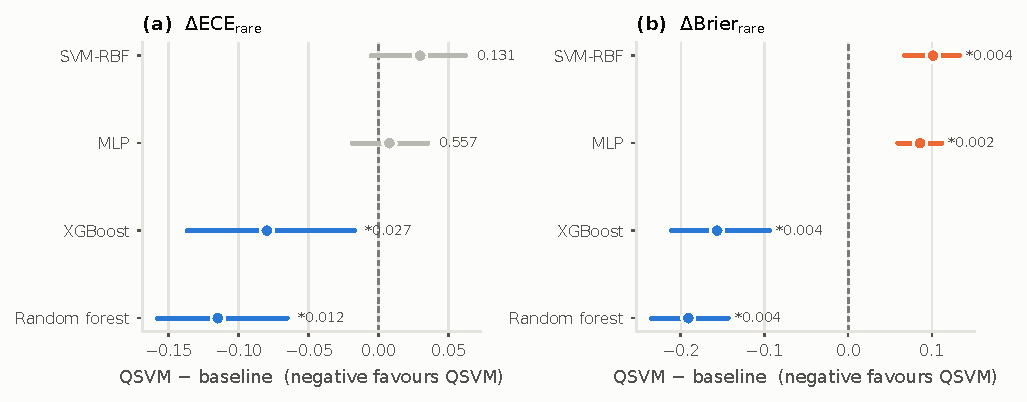
\includegraphics[width=\columnwidth]{figs/fig2_paired.pdf}
  \caption{Paired differences in calibration error, quantum kernel minus
  baseline, with bootstrap confidence intervals and Holm-corrected $p$.
  Blue favours the quantum kernel, orange the baseline, grey is
  inconclusive.}
  \label{fig:paired}
\end{figure}

\subsection{Calibration against the tree ensembles}
The quantum kernel is better calibrated than both tree ensembles in every
setting tested. On NSL-KDD the paired difference is $\pdNslRf$
$[\pdNslRfLo,\pdNslRfHi]$ ($p_{\text{Holm}}=\pdNslRfHolm$, $d_z=\pdNslRfDz$)
against Random Forest and $\pdNslXgb$ $[\pdNslXgbLo,\pdNslXgbHi]$
($p_{\text{Holm}}=\pdNslXgbHolm$) against XGBoost. On UNSW-NB15 at the
selected width the same comparisons give $\pdUnswSixRf$
($p_{\text{Holm}}=\pdUnswSixRfHolm$, $d_z=\pdUnswSixRfDz$) and
$\pdUnswSixXgb$ ($p_{\text{Holm}}=\pdUnswSixXgbHolm$), and at
$\plegacyQubits$ qubits $\pdUnswFourRf$ and $\pdUnswFourXgb$. Eight of eight
comparisons are corrected-significant in the quantum kernel's favour, and
the effect is far larger on UNSW-NB15 than on NSL-KDD.

\subsection{Where the quantum kernel does not lead}
The MLP is better calibrated than the quantum kernel in every setting
($\pdNslMlp$ on NSL-KDD, $p_{\text{Holm}}=\pdNslMlpHolm$; $\pdUnswSixMlp$ on
UNSW-NB15, $p_{\text{Holm}}=\pdUnswSixMlpHolm$), and we report this as
prominently as the wins. Against the classical RBF kernel the outcome is
dataset-dependent: on NSL-KDD the RBF kernel is ahead ($\pdNslRbf$,
$p_{\text{Holm}}=\pdNslRbfHolm$), while on UNSW-NB15 the comparison is
inconclusive at both widths ($p_{\text{Holm}}=\pdUnswSixRbfHolm$ at
$\punswQubits$ qubits). The claim this paper supports is a claim about tree
ensembles, not a claim that a quantum kernel is the most reliable model
available.

\begin{figure}[t]
  \centering
  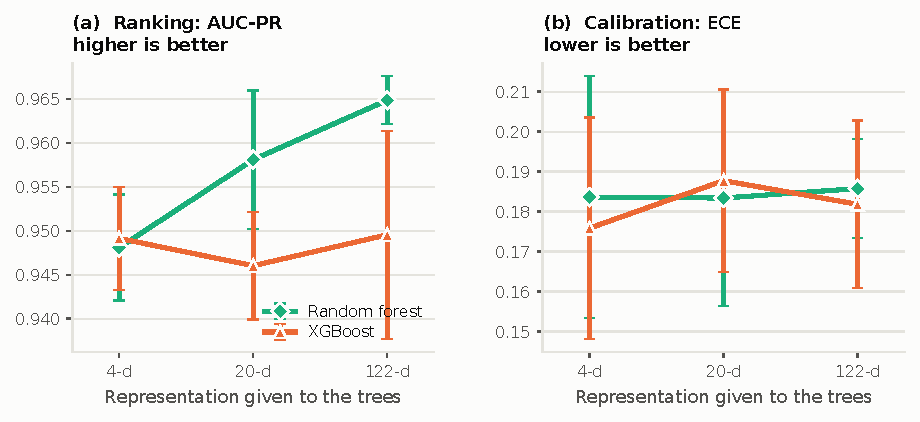
\includegraphics[width=\columnwidth]{figs/fig4_refarm.pdf}
  \caption{Giving the tree ensembles a richer representation, with every
  hyper-parameter held fixed. Ranking improves; calibration gets worse.}
  \label{fig:refarm}
\end{figure}

\subsection{Are the tree baselines handicapped?}
The trees share the quantum kernel's low-dimensional representation, which
invites the objection that they are compared in a form that suits them
badly. We repeat them on the $\prefKTwentyDims$ selected features and on the
full $\prefFullDims$ one-hot encoding, holding every hyper-parameter fixed
so that only the representation changes.

More features do not make the trees better calibrated. Random Forest's
calibration error moves from $\prefPcaRfEceFull$ to $\prefFullRfEceFull$ and
XGBoost's from $\prefPcaXgbEceFull$ to $\prefFullXgbEceFull$ --- slightly
worse in both cases, and in neither case enough to approach the quantum
kernel. Ranking moves the other way and by a larger margin: Random Forest's
AUC-PR improves from $\prefPcaRfAucPr$ to $\prefFullRfAucPr$. The point is
not that the richer representation harms the trees much; it is that it does
not help their calibration at all, so the comparison in
Table~\ref{tab:main} is made in the trees' most favourable calibration
setting rather than a cramped one.

\begin{figure}[t]
  \centering
  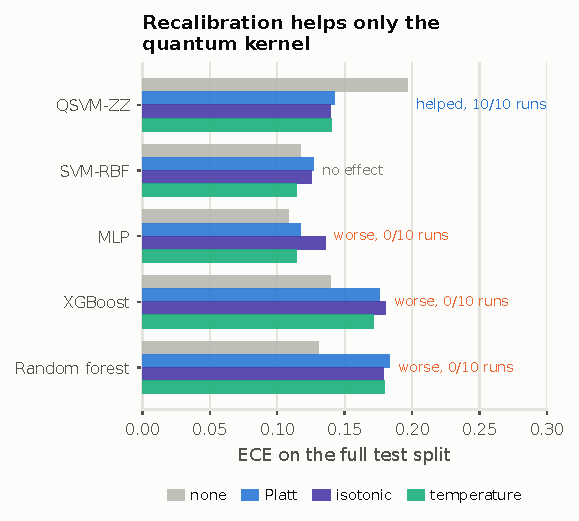
\includegraphics[width=\columnwidth]{figs/fig3_platt.pdf}
  \caption{Post-hoc recalibration helps the quantum kernel and degrades
  every other model.}
  \label{fig:platt}
\end{figure}

\subsection{When post-hoc recalibration helps}
Platt scaling reduces the quantum kernel's calibration error from
$\pQsvmPlattBefore$ to $\pQsvmPlattAfter$ ($\pQsvmPlattDelta$) and is the
only model of the five it helps: Random Forest moves by $\pRfPlattDelta$ and
XGBoost by $\pXgbPlattDelta$, both worse, and the classical SVM degrades
slightly ($\pRbfPlattDelta$).

This is not an artefact of choosing a logistic map. Isotonic regression and
temperature scaling give the same picture: on the quantum kernel all three
land within a narrow band ($\pcalQsvmPlatt$, $\pcalQsvmIso$,
$\pcalQsvmTemp$ against $\pcalQsvmNone$ uncalibrated), while on both tree
ensembles all three are worse than leaving the native probability alone
(Random Forest $\pcalRfNone$ uncalibrated against $\pcalRfIso$ isotonic).

\subsection{Ranking is not reliability}
The tree ensembles hold the best ranking and the worst calibration, on both
corpora. Ranking quality and probability quality are separate axes, and a
detector deployed on a probability threshold is governed by the second.

%==============================================================================
\section{Limitations}\label{sec:limits}

% TODO(tac gia): mo rong.
The calibration estimate remains a binned one and is sensitive to bin count.
The recalibrators are fitted on the training split, which is in-sample for
models that can memorise it; a held-out calibration split may change the
recalibration result, though not the ordering in Table~\ref{tab:main}. The
quantum kernel is evaluated by exact statevector simulation, so shot and
device noise are not represented. Both corpora are offline benchmark
captures.

%==============================================================================
\section{Conclusion}\label{sec:conclusion}

% TODO(tac gia).

\begin{thebibliography}{1}
% TODO: giu danh muc cua ban da nop.
\end{thebibliography}

\end{document}
